\subsection{Circuito di condizionamento}
\subsubsection{Obiettivo}
Per adattare il segnale del traduttore al circuito di misura e conversione
trattato nella sezione \ref{sec:adc} è necessario passare da una forma d'onda
come quella mostrata in figura \ref{fig:sign_trasd} ad un segnale sinusoidale
con $V_{eff(Max)} = 5V$ (fondoscala dell'adc) senza componente continua come
mostrato in figura \ref{fig:sign_adattato}.

\begin{figure}[H]
    \centering
    \begin{subfigure}{0.49\textwidth}
        \centering
        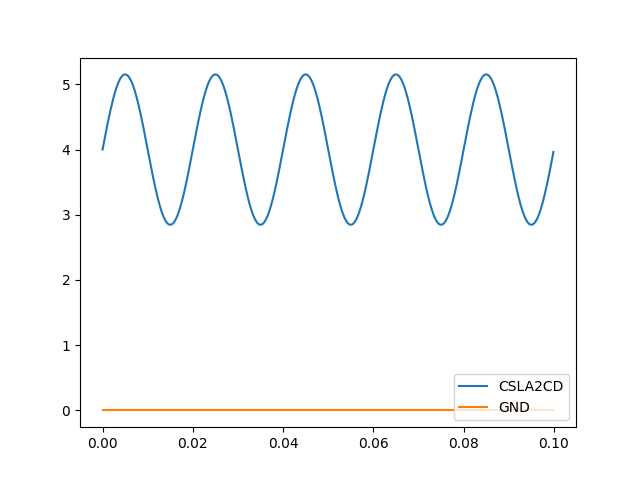
\includegraphics[scale=0.5]{corrente/sign_trasd.png}
        \caption{Uscita CSLA2CD}
        \label{fig:sign_trasd}
    \end{subfigure}
    \begin{subfigure}{0.49\textwidth}
        \centering
        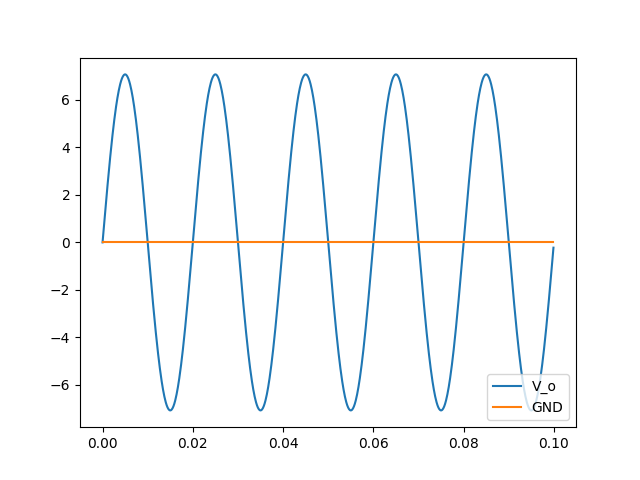
\includegraphics[scale=0.5]{corrente/sign_adattato.png}
        \caption{Segnale condizionato}
        \label{fig:sign_adattato}
    \end{subfigure}
    \caption{Segnale di partenza e condizionato in condizioni di corrente massima}
\end{figure}

\subsubsection{Schema a blocchi}

\begin{figure}[H]
    \centering
    \begin{tikzpicture}[thick, scale=1.2, every node/.style={scale=1.2}]
        \node[
            draw,
            circle,
            minimum size=0.7cm
        ](sum) at (0,0){};

        \node[
            draw,
            below=1cm of sum,
            minimum width=1.5cm,
            minimum height=1cm
        ](ref){$V_{ref}$ (LM336)};

        \node[
            draw,
            right=2cm of sum,
            minimum width=2cm,
            minimum height=1.5cm
        ](gain){$Kp$ (INA111)};

        \draw [-stealth](-3,0) -- (sum.west)
        node[near end,above]{+}
        node[at start ,above]{$V_{sens}$};

        \draw [-stealth](ref.north)--(sum.south)
        node[near end, left]{-};

        \draw [-stealth](sum.east)--(gain.west);

        \draw [-stealth](gain.east) -- ++ (2,0)
        node[near end, above]{$V_{out}$};
    \end{tikzpicture}
\end{figure}

\subsubsection{Tensione di riferimento}
Per rimuovere l'offset di $V_{cc}/2 = 4V$ introdotto dal trasduttore, è stata
applicata all'ingresso invertente dell'amplificatore per strumentazione una tensione di
riferimento di pari valore generata da un LM336z2.5 opportunamente amplificato
secondo lo schema che segue.

\begin{figure}[H]
    \centering
    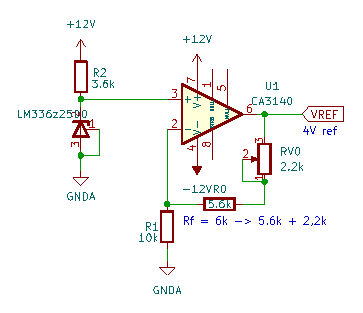
\includegraphics[scale=1.5]{corrente/ref.eps}
    \caption{Circuito di generazione tensione di riferimento}
\end{figure}

\subsubsection{Condizionamento con amplificatore per strumentazione}
Un amplificatore per strumentazione \textbf{INA111} è utilizzzato per rimuove la
tensione di offset e amplificare in modo adeguato il segnale per riportarlo al
caso in figura \ref{fig:sign_adattato}

\begin{figure}[H]
    \centering
    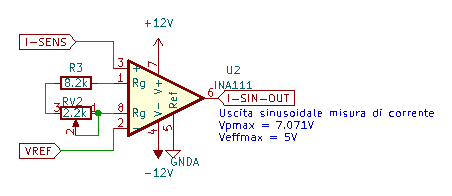
\includegraphics[scale=1.5]{corrente/ina.eps}
    \caption{Circuito di condizionamento}
\end{figure}

